\begin{figure}[h!]
	\centering
	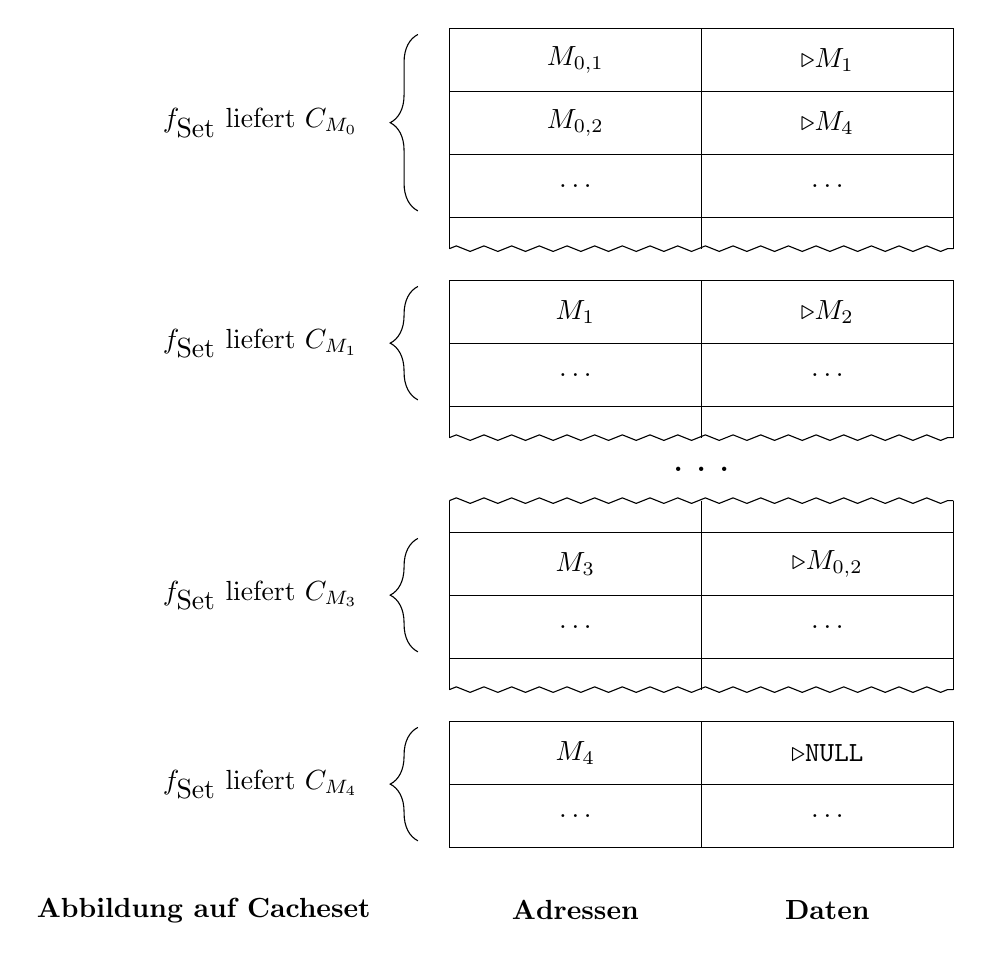
\begin{tikzpicture}[scale=0.8]
% === erste Cacheline
\draw (0,47)--(0,46.5); \draw (4,47)--(4,46.5); \draw (8,47)--(8,46.5);
\draw [decoration={zigzag,segment length=10pt, amplitude=1pt},decorate] (0,46.5)--(8,46.5);

\draw (0,47) rectangle node[] {\textbf{$\dots$}} (4,48); 
\draw (4,47) rectangle node[] {\textbf{$\dots$}}(8,48);

\draw (0,48) rectangle node[] {\textbf{$M_{0,2}$}} (4,49); 
\draw (4,48) rectangle node[] {\textbf{$\triangleright M_4$}}(8,49);

\draw (0,49) rectangle node[] {\textbf{$M_{0,1}$}} (4,50); 
\draw (4,49) rectangle node[] {\textbf{$\triangleright M_1$}} (8,50);

\draw [decorate,decoration={brace,amplitude=10pt}]
(-0.5,47.1) -- (-0.5,49.9) node [black,midway,xshift=-2cm] {$f_{\textrm{Set}}$ liefert $C_{M_0}$};

% === zweite Cacheline

\draw (0,45) rectangle node[] {\textbf{$M_{1}$}} (4,46); 
\draw (4,45) rectangle node[] {\textbf{$\triangleright M_2$}}(8,46);
\draw (0,44) rectangle node[] {\textbf{$\dots$}} (4,45); 
\draw (4,44) rectangle node[] {\textbf{$\dots$}}(8,45);

\draw (0,44)--(0,43.5); \draw (4,44)--(4,43.5); \draw (8,44)--(8,43.5);
\draw [decoration={zigzag,segment length=10pt, amplitude=1pt},decorate] (0,43.5)--(8,43.5);
\draw [decorate,decoration={brace,amplitude=10pt}]
(-0.5,44.1) -- (-0.5,45.9) node [black,midway,xshift=-2cm] {$f_{\textrm{Set}}$ liefert $C_{M_1}$};

% === Lücke
\node at (4,43) {\textbf{. . .}};

% === vorletzte Cacheline
\draw (0,42.5)--(0,42); \draw (4,42.5)--(4,42); \draw (8,42.5)--(8,42);
\draw [decoration={zigzag,segment length=10pt, amplitude=1pt},decorate] (0,42.5)--(8,42.5);

\draw (0,41) rectangle node[] {\textbf{$M_{3}$}} (4,42); 
\draw (4,41) rectangle node[] {\textbf{$\triangleright M_{0,2}$}}(8,42);
\draw (0,40) rectangle node[] {\textbf{$\dots$}} (4,41); 
\draw (4,40) rectangle node[] {\textbf{$\dots$}}(8,41);

\draw (0,40)--(0,39.5); \draw (4,40)--(4,39.5); \draw (8,40)--(8,39.5);
\draw [decoration={zigzag,segment length=10pt, amplitude=1pt},decorate] (0,39.5)--(8,39.5);
\draw [decorate,decoration={brace,amplitude=10pt}]
(-0.5,40.1) -- (-0.5,41.9) node [black,midway,xshift=-2cm] {$f_{\textrm{Set}}$ liefert $C_{M_3}$};

% === letzte Cacheline
\draw (0,38) rectangle node[] {\textbf{$M_{4}$}} (4,39); 
\draw (4,38) rectangle node[] {\textbf{$\triangleright$}\texttt{NULL}}(8,39);
\draw (0,37) rectangle node[] {\textbf{$\dots$}} (4,38); 
\draw (4,37) rectangle node[] {\textbf{$\dots$}}(8,38);
\draw [decorate,decoration={brace,amplitude=10pt}]
(-0.5,37.1) -- (-0.5,38.9) node [black,midway,xshift=-2cm] {$f_{\textrm{Set}}$ liefert $C_{M_4}$};

%Beschriftung
\node at (-3.9,36) {\textbf{Abbildung auf Cacheset}}; \node at (2,36) {\textbf{Adressen}}; \node at (6,36) {\textbf{Daten}};
	\end{tikzpicture}
	\caption{Speicherlayout für Pointer-Chasing der Zugriffssequenz\\ $O_{S,1} = (M_0,\; M_1,\; M_2,\; M_3,\; M_0,\; M_4)$}
	\label{cacheLayout}
\end{figure}
